%%%%%%%%%%%%%%%%%%%%%%%%%%%%%%%%%%%%%%%%%%%%%%%%%%%%%%%%%%%%%%%%
\begin{frame}[fragile]
\frametitle{\# 226: The Price of Distraction}


 \begin{center}

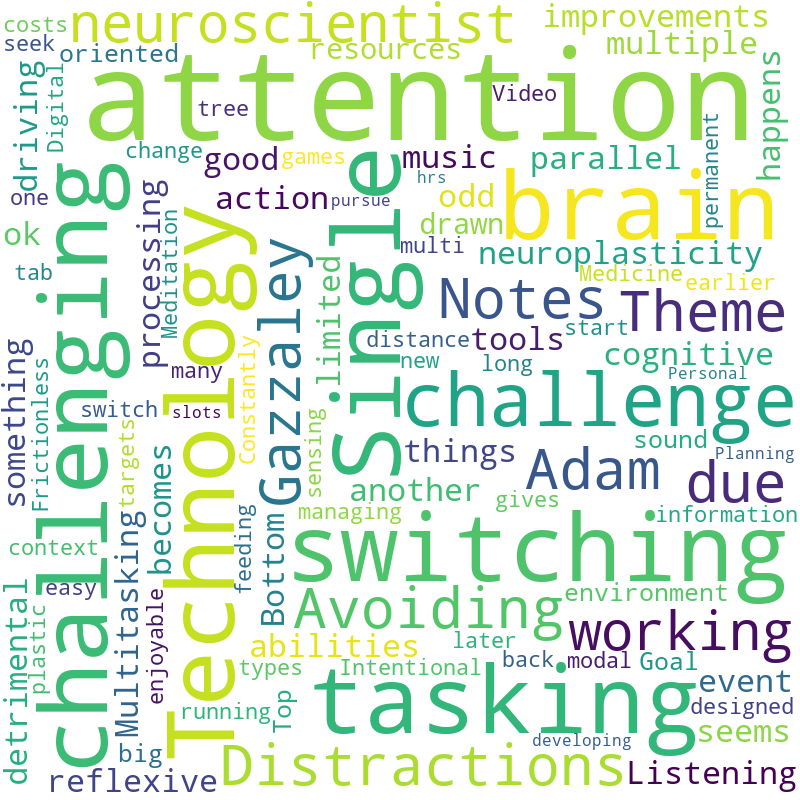
\includegraphics[width=0.6\linewidth,keepaspectratio]{images/Review_Podcast_MakingSense_226_PriceOfDistraction}
\end{center}

\end{frame}

%%%%%%%%%%%%%%%%%%%%%%%%%%%%%%%%%%%%%%%%%%%%%%%%%%%%%%%%%%%%%%%%
\begin{frame}[fragile]
\frametitle{\# 226: The Price of Distraction}

 A Conversation with Adam Gazzaley

\begin{itemize}
\item Theme: Avoiding Distractions due to Technology
\item Adam Gazzaley, neuroscientist working on neuroplasticity and tools for improvements of cognitive abilities
\item Multitasking: we like and good at doing multiple things, but should not be parallel-processing. 
\item Listening to music and another reflexive action like driving seems ok, but if there is something odd that happens, then switching the attention to that event becomes challenging and could be detrimental.
\item Bottom up attention: limited brain resources are drawn, by environment, like big sound.
\item Top down attention: Goal oriented. Intentional.
\end{itemize}


\end{frame}

%%%%%%%%%%%%%%%%%%%%%%%%%%%%%%%%%%%%%%%%%%%%%%%%%%%%%%%%%%%%%%%%
\begin{frame}[fragile]
\frametitle{\# 226: The Price of Distraction}

\begin{itemize}
\item Constantly managing, both types. Switching costs to get the earlier context.
\item Technology is designed to seek your attention. Each tab, gives you new information tree, and there are many of them, easy to switch. Frictionless.
\item Single tasking - challenging to start with but enjoyable later, like long distance running.
\item Digital Medicine: challenge brain targets for permanent/plastic change. Meditation is one.Video games multi modal sensing and then feeding back in to developing challenges.
\item Future of Technology: chip in body for extreme cases.
\end{itemize}

[Personal: Planning to pursue single-tasking in 2 hrs slots]
\end{frame}



%%%%%%%%%%%%%%%%%%%%%%%%%%%%%%%%%%%%%%%%%%%%%%%%%%%%%%%%%%%%%%%%
\begin{frame}[fragile]
\frametitle{\# 227: Knowing The Mind}


 \begin{center}

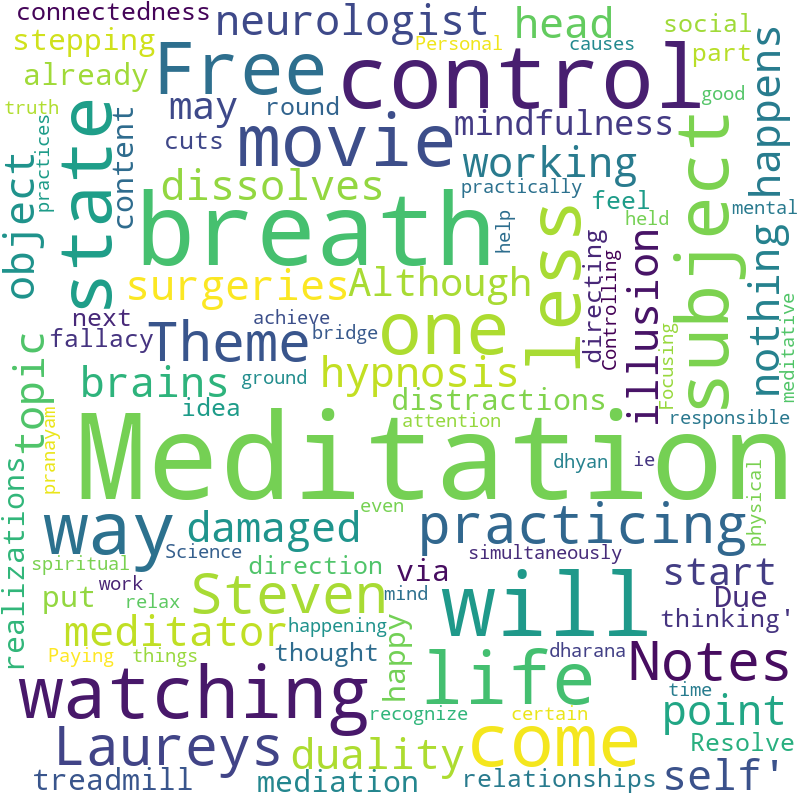
\includegraphics[width=0.6\linewidth,keepaspectratio]{images/Review_Podcast_MakingSense_227_KnowingTheMind}
\end{center}

\end{frame}

%%%%%%%%%%%%%%%%%%%%%%%%%%%%%%%%%%%%%%%%%%%%%%%%%%%%%%%%%%%%%%%%
\begin{frame}[fragile]
\frametitle{\# 227: Knowing The Mind}

 A Conversation with Steven Laureys

\begin{itemize}
\item Theme: Meditation
\item  Steven Laureys, a practicing neurologist working on damaged brains, surgeries under hypnosis.
\item  Meditation: subject-object duality is an illusion. At one point, the meditator and the topic of meditation dissolves into one. No control, just happens.
\item  There is nothing watching, no `self' in head. Although you may start with watching breath, but the state comes when mindfulness has no subject.
\item  Meditation: doing less, stepping out of the treadmill.
\item  Due to realizations via mediation, you already are happy/content and then you put that in relationships, social connectedness and not the other way round.
\end{itemize}


\end{frame}

%%%%%%%%%%%%%%%%%%%%%%%%%%%%%%%%%%%%%%%%%%%%%%%%%%%%%%%%%%%%%%%%
\begin{frame}[fragile]
\frametitle{\# 227: Knowing The Mind}

\begin{itemize}
\item Meditation cuts the idea that you are 'thinking'. There is no Free will.
\item  Free Will: You don't have control on what thought will come next. You feel you are directing the movie, but the direction itself is part of the movie.
\item  Resolve the fallacy by doing both simultaneously ie have a good life, do work, achieve things, at the same time recognize that its just happening on its own [but practically in life, you are held responsible for what you do].
\item  Science is ground truth for even spiritual practices. Paying attention certain ways only causes meditation.
\end{itemize}

[Personal: Breath (pranayam) is the bridge from physical to mental. Controlling breath can control mind, relax it. Focusing on breath (dharana) can help get into meditative state (dhyan)]
\end{frame}

%%%%%%%%%%%%%%%%%%%%%%%%%%%%%%%%%%%%%%%%%%%%%%%%%%%%%%%%%%%%%%%%
\begin{frame}[fragile]
\frametitle{\# 228: Doing Good}


 \begin{center}

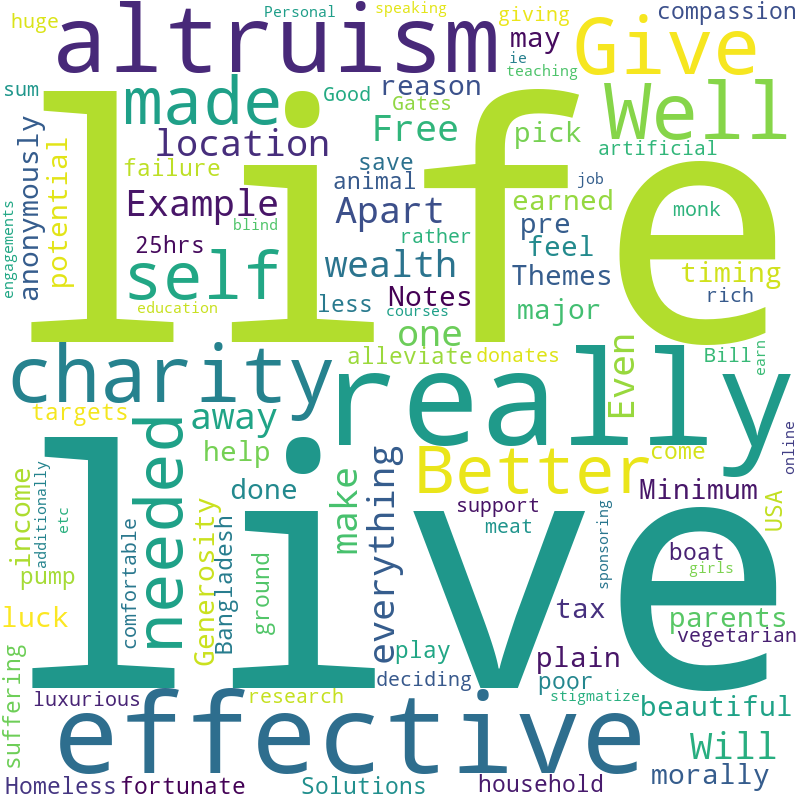
\includegraphics[width=0.6\linewidth,keepaspectratio]{images/Review_Podcast_MakingSense_228_DoingGood}
\end{center}

\end{frame}

%%%%%%%%%%%%%%%%%%%%%%%%%%%%%%%%%%%%%%%%%%%%%%%%%%%%%%%%%%%%%%%%
\begin{frame}[fragile]
\frametitle{\# 228: Doing Good}

 A Conversation with William MacAskill

% \begin{columns}[T] % align columns
% \begin{column}{.48\linewidth}
\begin{itemize}
\item Themes: Generosity, effective altruism.
\item Minimum 10\% of pre-tax income to most effective charity ("Give-Well")
\item  Better if done anonymously? Not really!! Taking public pledge.
\item  Altruism needed? Be self-made?
\item  You didn't pick location, parents, timing and plain luck. So, not really ``self''-made. Like Will in Free-Will may not be really be Free.
\item  Even if you feel you have earned it, why not help? Have compassion for less fortunate.
\end{itemize}


\end{frame}

%%%%%%%%%%%%%%%%%%%%%%%%%%%%%%%%%%%%%%%%%%%%%%%%%%%%%%%%%%%%%%%%
\begin{frame}[fragile]
\frametitle{\# 228: Doing Good}


\begin{itemize}
\item Solutions should come from the ground. Example of failure: 25hrs on play-pump needed for one household.
\item  What are targets for charity? Homeless in USA or poor in Bangladesh?
\item  Make life boat better, to save more.
\item  To alleviate animal suffering: be vegetarian, support artificial meat research
\item  Good example: Bill Gates lives a luxurious life and donates huge sum as well, rather than deciding to live like a monk while giving away everything else. Even other rich are comfortable doing same. Don't stigmatize wealth.
\end{itemize}


[Personal: Apart from sponsoring blind girls education, additionally, I give away everything I earn apart from my job, ie from my speaking engagements, online courses, teaching, etc.]
\end{frame}

% %%%%%%%%%%%%%%%%%%%%%%%%%%%%%%%%%%%%%%%%%%%%%%%%%%%%%%%%%%%%%%%%
% \begin{frame}[fragile]
% \frametitle{Prelude}

% \begin{columns}[T] % align columns
% \begin{column}{.48\textwidth}
% \begin{itemize}
% \item Mind is divided into 4 sections
	% \begin{itemize}
	% \item Section 1 : Brain
	% \item Section 2 a: RAS
	% \item Section 2 b: CCS
	% \item Section 3 : Extra Sensory Perceptions
	% \item Section 4 : Soul (atman)
	% \end{itemize}
% \item RAS:
% \item CCS: Critical Certain Stage
% \item Lower Dimension: 1, 2a
% \item Higher Dimension: 2b, 3, 4
% \end{itemize}
% \end{column}%
% \hfill%
% \begin{column}{.48\textwidth}
 % \begin{center}
% \includegraphics[width=0.9\linewidth,keepaspectratio]{images/zenyoga1}
% \end{center}

% \end{column}%
% \end{columns}
% \end{frame}

% %%%%%%%%%%%%%%%%%%%%%%%%%%%%%%%%%%%%%%%%%%%%%%%%%%%%%%%%%%%%%%%%
% \begin{frame}[fragile]
% \frametitle{Section 2a}
% \begin{itemize}
% \item Intercepts flow from physical body, senses.
% \item Adjusts/tones-down/accentuates and sends to thalamus to cortex for decision making.
% \item Thus body can report bodily disorders to brain directly without consulting conscious mind.
% \item This covers all unconscious/autonomous functions.
% \end{itemize}
% \end{frame}

% %%%%%%%%%%%%%%%%%%%%%%%%%%%%%%%%%%%%%%%%%%%%%%%%%%%%%%%%%%%%%%%%
% \begin{frame}[fragile]
% \frametitle{Section 2b}
% Concentration, Meditation, Intuition.

 % \begin{center}
% \includegraphics[width=0.35\linewidth,keepaspectratio]{images/zenyoga2}
% \end{center}

% Goal: Cross the divide (no-mans-land) and go to CCS and further.

% \end{frame}
